\vspace{-6ex}
\noindent\rule{\linewidth}{0.5pt}\vspace{-2ex}
\begin{multicols}{2}
\section*{Chapter One - Vector spaces}
\begin{definition}
A \textbf{field} $F$ is a set with functions $+$ and $\times$ such that $G_+:=(F,+)$ and $G_\times:=(F\setminus\{0_F\},\times)$ are abelian groups with $\text{id}_{G_\times}=1_F$, $\text{id}_{G_+}:=0_F$ and for $\lambda,\mu,\nu\in F$ we have that $\lambda(\mu+\nu) = \lambda\mu + \lambda\nu$.
\end{definition}

\begin{definition}
A \textbf{vector space} $V$ over a field $F$ is a pair $(V,\dot{+})$ where $V$ is a set and $\dot{+}:F\times V\to V:(\lambda,\v)\mapsto\lambda\v$ is a map where for $\lambda,\mu\in F$ and $\u,\v\in V:$\vspace{-2ex}
    \begin{multicols}{2}
    \begin{itemize}
        \item{$\lambda(\u+\v) = \lambda\u + \lambda\v$,}
        \item{$(\lambda+\mu)\v = \lambda\v + \mu\v$,}
        \item{$\lambda(\mu\v)=(\lambda\mu)\v$,}
        \item{$1_F\v=\v$.}
    \end{itemize}
    \end{multicols}
\end{definition}

\begin{theorem}[1.2.2]
If $V$ is a vector space and $\v\in V$ , then $0\v = \vec{0}$.
\end{theorem}
\begin{proof}
$0\v = (0 + 0)\v = 0\v + 0\v \Rightarrow  \vec{0} = 0\v$.
\end{proof}

\begin{definition}
A subset $U\subseteq V$ of a vector space $V$ is a \textbf{vector subspace} if $U$ contains $\vec{0}$ and  $\u,\v\in U,\lambda\in F\Rightarrow \u+\v\in U$ and $\lambda\u \in U$.
\end{definition}

\begin{theorem}
Let $T\subseteq V$, then $\langle T\rangle := \{\sum_{\alpha_i\in F}\alpha_i\v_i : \v_i\in T\}$ is a subspace of $V$. If $V=\langle T\rangle$ then $T$ is a \textbf{generating set} of $V$.
\end{theorem}

\begin{definition}
A subset $L$ of a vector space $V$ is \textbf{linearly independent} if for all pairwise different vectors $\v_1,\dots,\v_r \in L$ and arbitrary scalars $\alpha_1,\dots,\alpha_r\in F$, we have that $\alpha_1\v_1+\dots+\alpha_r\v_r = \vec{0} \implies \forall i: \alpha_i = 0$.
\end{definition}

\begin{definition}
A \textbf{basis} of a vector space $V$ is a linearly independent generating set of $V$.
\end{definition}

\begin{theorem}[1.5.11]
Let $V$ be a vector space over a field $F$ and $\v_1,\dots,\v_r\in V$ vectors. The family $(\v_i)_{1\leq i\leq r}$ is a basis of $V$ \textit{if and only if} $\phi:F^r\to V:(\alpha_1,\dots,\alpha_r)\mapsto \sum_{i=1}^r\alpha_i\v_i$ is a bijection.
\end{theorem}
\begin{proof}
$(\v_i)_{1\leq i\leq r}$ is a generating set $\Leftrightarrow \phi$ is a surjection $F^r\to V$.

$(\v_i)_{1\leq i\leq r}$ is linearly independent $\Leftrightarrow \phi$ is a injection $F^r\to V$.

$(\v_i)_{1\leq i\leq r}$ is a basis $\Leftrightarrow \phi$ is a bijection $f^r\to V$.
\end{proof}

\begin{theorem}[1.5.13]
Let $V$ be a finitely generated vector space over a field $F$, then $V$ has a basis.
\end{theorem}

\begin{theorem}
If $V$ is a vector space, $L\subset V$ a linearly independent subset and $E\subseteq V$ a generating set, then $|L|\leq |E|$.
\end{theorem}

\begin{theorem}[Exchange Lemma] 
Let $M\subseteq E\subseteq V$ be such that $M$ is linearly independent and $V=\langle E\rangle$. If $\vec{w} \in V \setminus M$ is such that $M\cup \{\vec{w}\}$ is linearly independent, then $\exists\vec{e} \in E \setminus M$ such that $V=\langle (E \setminus \{\vec{e}\}) \cup \{\vec{w}\}\rangle$. Thus \textbf{any two bases for $V$ must have the same cardinality}.
\end{theorem}
% \begin{proof}
% Express $\vec{w}$ in terms of the generating set $E$ so that $\vec{w}=\sum_{i=1}^{|E|}\alpha_i\vec{e}_i$ and WLOG assume that $\vec{e}_1\notin M$ so that $\vec{e}_1 = \alpha_1^{-1}(\vec{w}-\alpha_2\vec{e}_2-\dots-\vec{e}_{|E|})$. 
% \end{proof} %%UNCOMMENT%%

\begin{definition}
The \textbf{dimension} of a vector space $V$ is the cardinality of any basis of $V$ (by the exchange-lemma this is independent of choice of basis).
\end{definition}

\begin{theorem}[The Dimension Theorem]
Let $V$ be a vector space with subspaces $U, W\subseteq V$. Then $\dim(U+V) + \dim(U\cap V) = \dim(U)+\dim(V)$.
\end{theorem}
\begin{proof}
Choose a basis $\vec{s}_1,\dots,\vec{s}_d$ of $U\cap W$ and extend it by the elements $\u_1,\dots,\u_r\in U$ to a basis of $U$ and then by the elements $\vec{w}_1,\dots,\vec{w}_t\in W$ to a basis of $U + W$. Then show that $\{\vec{s}_1,\dots,\vec{s}_d,zvec{w}_1,\dots,\vec{w}_t\}$ is a basis of $W$. It's linearly independent by construction, so show that it's generating.
\end{proof}

\begin{definition}
A mapping $f:V\to W$ between vector spaces $V,W$ is \textbf{linear} iff $\forall\u,\v\in V: f(\u+\v)=f(\u)+f(\v)$ and $\forall\lambda\in F: f(\lambda\v)=\lambda f(\v)$. If $f$ is bijective then it's an \textbf{isomorphism}, if $V=W$ then $f$ is an \textbf{endomorphism} and if both of these hold then $f$ is an \textbf{automorphism}.
\end{definition}

\begin{theorem}
Let $n\in\mathbb{N}$ and $V$ be vector space over a field $F$, then $V$ is isomorphic to $F^n$ iff $\dim(V)=n$.
\end{theorem}
% \begin{proof}
% Let $f:V\to W$ be a linear map, then $f$ is surjective $\Leftrightarrow f$ sends a generating set to a generating set and $f$ is injective $\Leftrightarrow f$ sends a L.I. subset to a L.I subset, so by 1.5.11 a vector space isomorphism sends a basis to a basis. Thus two isomorphic spaces have the same dimension. If $V$ has an ordered basis $B = (\v_1,\dots,\v_n)$, then the mapping $(\lambda_1,\dots, \lambda_n)\mapsto \lambda_1\v_1 +\dots+\lambda_n\v_n$ in Theorem 1.5.11 produces an isomorphism $F^n \to V$.
% \end{proof} %%UNCOMMENT%%

\begin{theorem}[1.7.8]
Let $V, W$ be vector spaces over $F$ and let $B\subset V$ be a basis. Then $\mathrm{Hom}(V,W)\ \tilde{\to}\ \mathrm{Maps}(B,W): f\mapsto f|_{B}$.
\end{theorem}
% \begin{proof}
% Just contract and expand linear maps $f:V\to W$ and $f|_B:B\to W$ by writing $\v$ in terms of the basis $B$, and show that they agree for all vectors $\v\in V$.
% \end{proof} %%UNCOMMENT%%

\begin{theorem}[1.7.9]
Let $f:V\to W$ be a linear map. If $f$ is injective then it has a left inverse, if $f$ is surjective then it has a right inverse.
\end{theorem}

\begin{definition}
Let $f:U\to V$ be linear. The \textbf{image} of $f$ is $\mathrm{im}(f) := f(V) =\{\v\in V:\exists\u\in U,\v = f(\u)\}$. The \textbf{kernel} of $f$ is the pre-image $\mathrm{ker}(f):=f^{-1}(\vec{0})$. We have $\mathrm{im}(f)\subseteq V$ and $\mathrm{ker}(f)\subseteq U$ are subspaces.
\end{definition}

\begin{theorem}[1.8.2]
A linear mapping $f : V \to W$ is injective if and only if its kernel is zero.
\end{theorem}

\begin{theorem}[Rank-Nullity]
Let $f : V \to W$ be a linear mapping between vector spaces. Then $\dim(V) = \dim(\ker(f)) + \dim(\mathrm{im}(f))$.
\end{theorem}

\end{multicols}

% BACKGROUND PICTURE :::
% \tikz[remember picture,overlay]
% {
% \node[opacity=0.4,inner sep=0pt] at (current page.center) {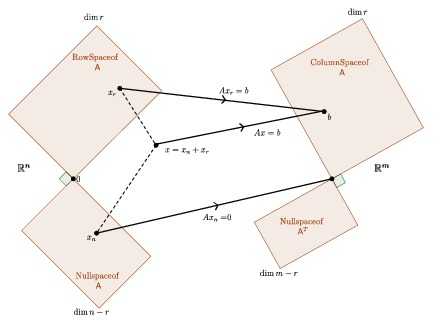
\includegraphics[width=\paperwidth]{subsp.jpg}};
% }\clearpage
